\documentclass{article}
\usepackage{graphicx} % for including images
\usepackage{float}    % for positioning tables and figures
\usepackage{listings} % for code listings

\begin{document}

\title{Sample Document 1}
\author{Lakindu Boteju}
\date{\today}

\maketitle

\section{Introduction}

This is a simple document to demonstrate a basic layout, including sections with headings, paragraphs, lists, a table, a code block and an image.

\vfill
\noindent
Text can be \textbf{BOLD}, \textit{Italic}, and \texttt{Monospace}.

\vfill
\noindent
We can also include ordered lists:
\begin{enumerate}
    \item Item 1
    \item Item 2
    \item Item 3
\end{enumerate}

\vfill
\noindent
And unordered lists:
\begin{itemize}
    \item Item 1
    \item Item 2
    \item Item 3
\end{itemize}

\subsection{Sub-heading}

In this section, we present a table with strict vertical and horizontal lines.

\begin{table}[H]
    \centering
    \begin{tabular}{|c|c|c|}
        \hline
        \textbf{Column 1} & \textbf{Column 2} & \textbf{Column 3} \\
        \hline
        Row 1, Col 1 & Row 1, Col 2 & Row 1, Col 3 \\
        \hline
        Row 2, Col 1 & Row 2, Col 2 & Row 2, Col 3 \\
        \hline
        Row 3, Col 1 & Row 3, Col 2 & Row 3, Col 3 \\
        \hline
    \end{tabular}
    \caption{Sample Table}
    \label{tab:sample_table}
\end{table}

\noindent
To create this document we used LaTeX,
which is a typesetting system that is widely used for
producing scientific and mathematical documents due to
its powerful handling of formulas and bibliographies.

\newpage

\subsection{Code Block and Image}
Here is a sample code snippet written in Python:

\begin{verbatim}
def hello_world():
    print("Hello, World!")

if __name__ == "__main__":
    hello_world() 
\end{verbatim}

\begin{figure}[H]
    \centering
    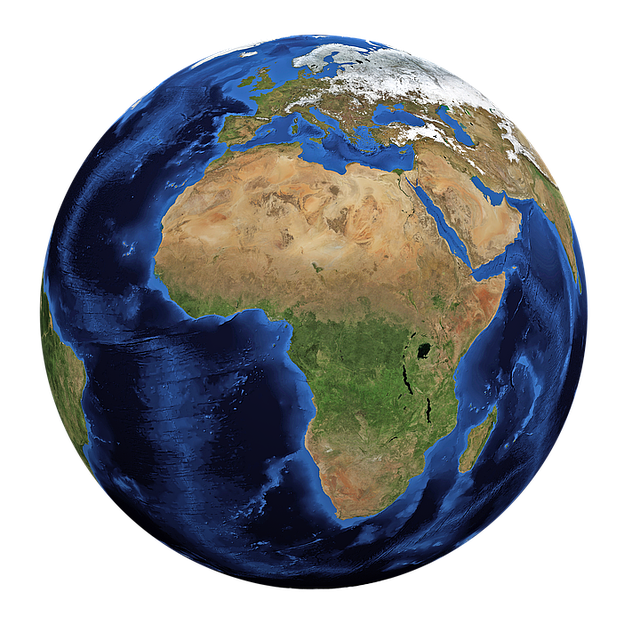
\includegraphics[width=0.5\textwidth]{earth.png} % Ensure this path is correct
    \caption{Sample Image}
    \label{fig:sample_image}
\end{figure}

\end{document}
